\subsection{Allgemein}
\subsubsection{IRemoteLoggerCheckPoint}\label{sec:IRemoteLoggerCheckPoint}
\begin{wrapfigure}[10]{r}[0cm]{150px} 
	\vspace{-12px}
	\centering
	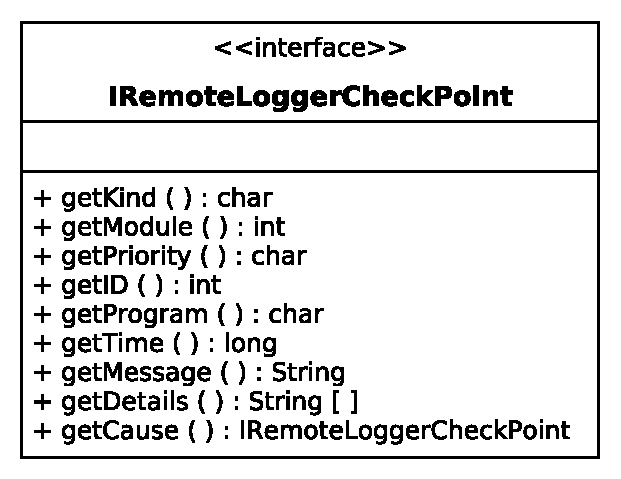
\includegraphics[width=140px]{../img/CD-IRemoteLoggerCheckPoint.eps}
	\caption{Aufbau eines \glqq IRemoteLoggerCheckPoint\grqq}
\end{wrapfigure}
\par Kapselt einen bereits vorhandenen CheckPoint. Enthält allerdings noch die Informationen über den Grund (getCause()), warum dieser CheckPoint aufgetreten ist. Somit wird eine Baumstruktur aus IRemoteLoggerCheckPoints erzeugt, mit der sich auftretende Fehler leicht identifizieren und beheben lassen.
\par Definition innerhalb von ADITO4: Ein CheckPoint setzt sich aus seiner Art, seinem Modul, seiner Priorität, seinem Identifier, seinem Programm und einer für den Benutzer lesbaren Meldung zusammen.
\begin{figure}[h]
	\vspace{20px}
	\begin{center}
		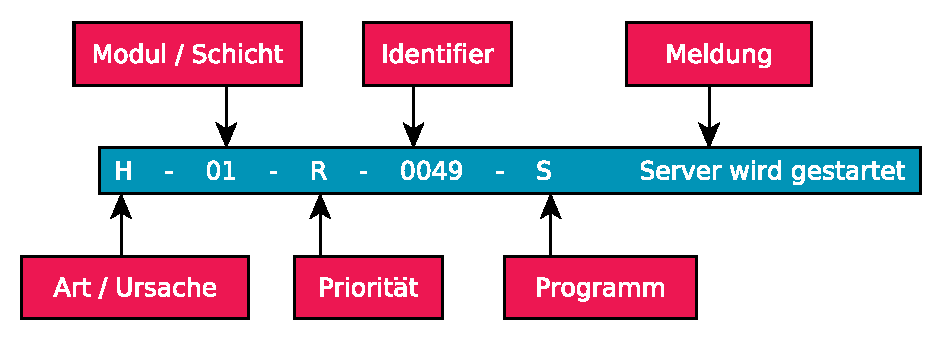
\includegraphics[width=0.8\textwidth]{../img/CheckPoint.eps}
		\vspace{4px}
		\caption{Aufbau eines CheckPoints in ADITO4}
	\end{center}
	\vspace{20px}
	\begin{tabularx}{\textwidth}{P{0.2\textwidth}|X}
		1. Art/Ursache & Gibt die Ursache des Fehlers an (Bug, Anwender- / Netzwerkfehler, etc.) \\
		\hline 2. Modul/Schicht & Gibt an, in welcher Schicht der Fehler aufgetreten ist (DB-, Kommunkations-, Kalenderschicht, etc.) \\
		\hline 3. Priorität & Gibt an, wie schwerwiegend die Meldung ist (A - Z, A = höchste Priorität) \\
		\hline 4. Identifier & Jede Meldung hat eine 4-stellige ID, die innerhalb eines Modules eindeutig ist \\
		\hline 5. Programm & Gibt an, welches Teilprogramm die Meldung verursachte (Client, Server, Designer, etc.) \\
		\hline 6. Meldung & Eine für den Benutzer lesbare Beschreibung \\
	\end{tabularx}
	\vspace{4px}
	\caption{Beschreibung der verschiedenen Bestandteile eines ADITO-CheckPoints}
	\label{fig:CheckPointParts}
\end{figure}
\newpage

\par \textit{\underline{DefaultRemoteLoggerCheckPoint}}
\par Als Datencontainer steht der \glqq DefaultRemoteLoggerCheckPoint\grqq\ zur Verfügung, um das o.g. Interface mit passenden Daten zu versorgen. Im Konstruktor erhält dieser ein Array aus CheckPoints und den zugehörigen Zeitstempel in Millisekunden. Die Arrayreihenfolge entspricht der zeitlichen Abfolge voneinander abhängigen Ereignissen (\glqq 'Meldung 1' verursacht durch 'Meldung 2' verursacht durch 'Meldung 3' ... \grqq). An der Stelle 0 enthält das Array den CheckPoint, dessen Daten durch die aktuelle \glqq DefaultRemoteLoggerCheckPoint\grqq-Instanz abgebildet werden sollen. An darauf folgender Stelle sind die Daten der übergeordneten CheckPoints, den \glqq Causes\grqq, zu finden. \\
Um den direkten Vorgänger instantiieren zu können benötigt man die Methode \glqq initCause(...)\grqq:
\begin{figure}[h]
	\begin{spacing}{0.75}
		\begin{javacode}[firstnumber=125]
protected IRemoteLoggerCheckPoint initCause(CheckPoint[] pTrace, long pTime)
{
  CheckPoint[] newTrace = Arrays.copyOfRange(pTrace, 1, pTrace.length);
  return pTrace.length == 1 ? null : new DefaultRemoteLoggerCheckPoint(newTrace, pTime);
}		\end{javacode}
	\end{spacing}
	\caption{initCause(...)-Methodenimplementierung innerhalb des \glqq DefaultRemoteLoggerCheckPoint\grqq}
\end{figure}
\vspace{10px}

\par \textit{\underline{TranslateableRemoteLoggerCheckPoint}}\vspace{-13px}
\begin{wrapfigure}[15]{r}[0cm]{180px}
	\vspace{10px} \hspace{5px}
	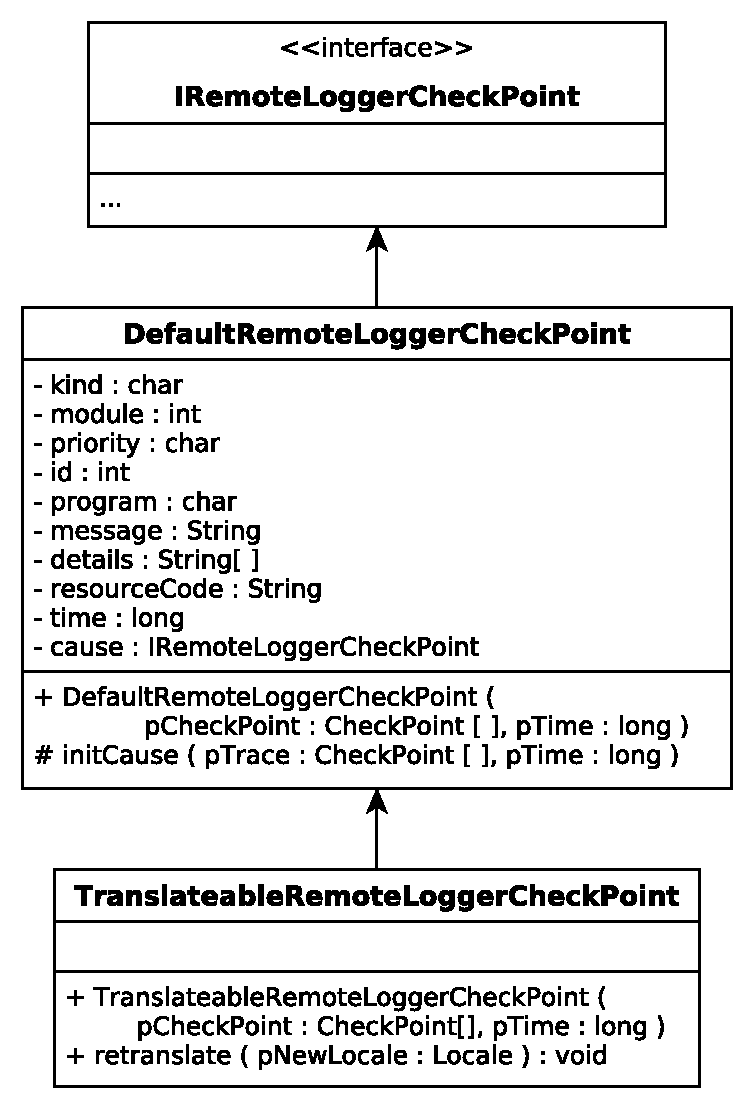
\includegraphics[width=175px]{../img/CD-TranslateableRemoteLoggerCheckPoint.eps}
	\caption{Klassenhierarchie des \glqq IRemoteLoggerCheckPoint\grqq}
\end{wrapfigure}
\par In der Theorie kann jeder verbundene Remote-Logger-Client eine andere Sprache besitzen, unabhängig der des Remote-Logger-Servers. Da dies mit o.g. Konstrukt noch nicht möglich ist, kommt hier der \glqq TranslateableRemoteLoggerCheckPoint\grqq\ ins Spiel. Dieser erweitert den \glqq DefaultRemoteLoggerCheckPoint\grqq\ um eine Übersetzungsfunktion.
\par Er enthält die Methode \glqq retranslate(pNewLocale : Locale)\grqq\ die aufgerufen werden kann, wenn die hinter dem CheckPoint liegende Meldung (siehe \prettyref{fig:CheckPointParts}, Punkt 6) in eine andere Sprache übersetzt werden soll. Falls diese in der gewünschten Sprache nicht vorliegt wird versucht, die englische Version zu laden. (Quellcode siehe Anhang  \prettyref{sec:CODE_TranslateableRemoteLoggerCheckPoint})

\newpage
\vspace{-2px}
\subsubsection{IRemoteLoggerCommand}\label{sec:IRemoteLoggerCommand}
\vspace{-2px}
\begin{wrapfigure}[6]{r}[0cm]{185px}
	\vspace{-10px} \hspace{5px}
	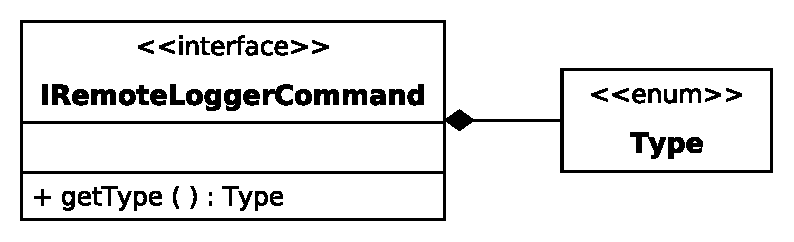
\includegraphics[width=180px]{../img/CD-IRemoteLoggerCommand.eps}
	\caption{Klassendiagramm des \glqq IRemoteLoggerCommand\grqq}
\end{wrapfigure}
\par Ein Remote-Logger-Kommando ist ein Befehl, der vom Remote-Logger-Client an den -Server gesendet wird um dort eine bestimmte Aktion auszuführen. Eine Instanz des IRemoteLoggerCommands muss vollständig serialisierbar sein und die kompletten Daten enthalten, die zur Durchführung der am Server hinterlegten Aktion benötigt werden (\prettyref{sec:CODE_IRemoteLoggerCommand}).
\vspace{-2px}
\par \textit{\underline{AuthorizationCommand}}
\vspace{2px}
\\ Mit Hilfe eines IRemoteLoggerCommands lässt sich ein Kommando zur Authorisierung eines Remote-Logger-Clients mittels beliebigen Login-Informationen (Username und Passwort, RSA-Schlüssel, etc.) am Remote-Logger-Server implementieren. Daraus ergeben sich mehrere Vorteile: Zum einen ist es durch diesen Authorisierungsvorgang gewährleistet, dass Unberechtigte keine Daten vom  Remote-Logger-Server erhalten. Zum anderen können die schon vorhandenen Login-Informationen des ADITO4-Managers dazu verwendet werden, denn dieser muss sich vor dem Verbinden mit dem ADITO4-Server ebenso authentifizieren (siehe \prettyref{fig:KommunikationServerManager}).
\vspace{-2px}
\par \textit{\underline{LanguageCommand}}
\vspace{2px}
\\ Ein weiteres Kommando stellt das \glqq LanguageCommand\grqq\ dar. Dadurch ist es möglich, die Sprache, in der etwaige CheckPoint-Meldungen übersetzt werden, spezifisch für jeden Remote-Logger-Client separat festzulegen.

\vspace{-2px}
\subsubsection{ObjectInputStreamConsumer} \label{sec:ObjectInputStreamConsumer}
\vspace{-2px}
\begin{wrapfigure}[12]{r}[0cm]{245px}
	\vspace{-23px} \hspace{5px}
	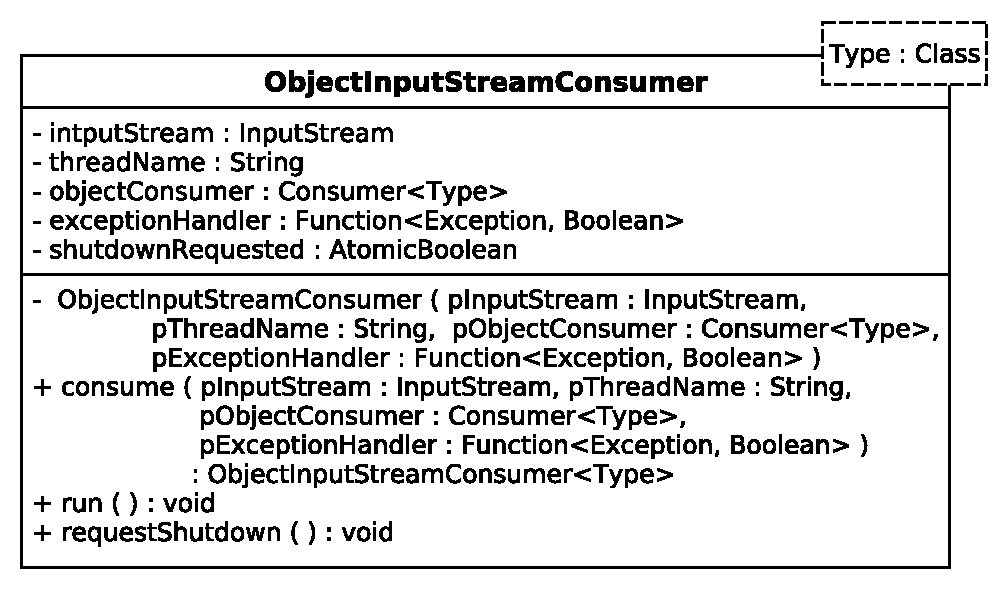
\includegraphics[width=240px]{../img/CD-ObjectInputStreamConsumer.eps}
	\caption{Aufbau des \glqq ObjectInputStreamConsumer\grqq}
\end{wrapfigure}
\par Der \glqq ObjectInputStreamConsumer\grqq\ kapselt einen übergebenen InputStream in einen ObjectInputStream und liest so lange Daten in einem isolierten Thread aus, bis entweder ein Herunterfahren von außen angefragt wurde oder ein interner Fehler beim Auslesen aufgetreten ist. Im Konstruktor erwartet diese Klasse neben dem auszulesenden Stream, dem gewünschten Threadnamen, einen Consumer zur Verarbeitung erfolgreich ausgelesener Objekte. Durch das Java-Generic wird bestimmt, welchen Typ die auszulesenden Objekte vorweisen. Zusätzlich kann eine Funktion übergeben werden die anhand von intern aufgetretenen Fehlermeldungen entscheiden kann, ob der Auslesevorgang erneut gestartet oder der StreamConsumer geschlossen werden soll. Mit der \glqq consume(...)\grqq\-Methode kann ein neuer ObjectInputStreamConsumer erstellt werden.
\par Der Hauptteil des o.g. Algorithmus ist in der \glqq run()\grqq\-Methode des Consumers implementiert:
\vspace{-5px}
\begin{figure}[h] 
\vspace{-4px}
    \centering
	\begin{spacing}{0.75}
		\begin{javacode}[firstnumber=56]	
  while(!shutdownRequested.get())
  {
    ...
    Object read;
    while (!shutdownRequested.get() && 
           (read = new ObjectInputStream(inputStream).readObject()) != null)
      objectConsumer.accept((Type) read);
    ...
  }\end{javacode}
	\end{spacing}
	\caption{Auslesen eines ObjectInputStreams im ObjectInputStreamConsumer}
\end{figure}